\documentclass[11pt]{article}
\usepackage[margin=2.4cm]{geometry}
\usepackage{amsmath,amssymb}
\usepackage{booktabs}
\usepackage{graphicx}
\usepackage{xcolor}
\usepackage{hyperref}
\usepackage{caption}
\usepackage{enumitem}
\usepackage{fancyhdr}
\usepackage{colortbl}

\definecolor{ok}{HTML}{1baf7a}
\definecolor{bad}{HTML}{e34948}
\definecolor{hl}{HTML}{2a78d6}

\pagestyle{fancy}
\fancyhf{}
\rhead{Pilot Study -- ``Why Did the Robot Hold Back?''}
\lhead{Optimization-Native Safety-Filter Explanations}
\rfoot{\thepage}

\title{\bfseries Pilot Feasibility Study\\[2pt]
\large Certified, Optimization-Native Explanations of Safety-Filter Interventions\\
in Deep Reinforcement Learning for Robotics}
\author{Prepared for: Bilal H. Abed-alguni \\ Department of Computer Science, Yarmouk University}
\date{September 21, 2026}

\begin{document}
\maketitle

\begin{abstract}
\noindent
Before committing to full-scale experiments (safe-RL benchmarks and a physical
robot demonstration), this pilot study tests the mathematical and empirical
core of the paper's claims on controlled, synthetic CBF-QP instances where the
ground truth is fully known and independently verifiable. Four experiments were
run: (1) numerical verification of the exact intervention-decomposition and
energy identities on 1{,}446 intervening instances; (2) attribution
faithfulness of the proposed deletion-interval method against three baselines
(naive violated-set, single-multiplier KKT, and a Shapley-value game-theoretic
attribution) on 10{,}872 constraint instances, evaluated against an exact
constraint-deletion ground truth; (3) validation of the closed-form and
two-sided-certificate counterfactuals against independent numerical solutions;
and (4) a test of whether the proposed conditioning indicator predicts
empirical explanation instability under perturbation. All four experiments
support the paper's central claims with no falsifying evidence found, and the
pilot additionally surfaces two concrete, previously implicit risks --
numerical sensitivity near degenerate active sets, and looseness of the
multi-obstacle counterfactual certificate under interacting constraints -- that
should be written up as limitations or addressed algorithmically. The
recommendation is to \textbf{proceed to full experiments}.
\end{abstract}

\tableofcontents

% ======================================================================
\section{Purpose and Scope}

The submitted manuscript introduces an \emph{optimization-native} explanation
framework for CBF-QP safety filters, with four theoretical contributions: an
exact intervention decomposition (Theorem 1), a deletion-based
filter-interventional faithfulness criterion (Theorem 2) together with
degeneracy-aware attribution intervals, certified counterfactual explanations
(closed-form for circular obstacles, two-sided certificates for multiple
constraints), and a stability/conditioning analysis. The paper's own
``Numerical Verification'' subsection (Sec.~VII-A) commits to reporting
identity errors of $10^{-8}$--$10^{-11}$ and zero mismatches across 800
deletion tests.

This pilot has one purpose: \textbf{decide whether the idea is worth the cost
of full experiments} (safe-RL simulation studies across multiple seeds and a
physical manipulator demonstration) \emph{before} that cost is incurred. It
therefore asks, on cheap, fully controlled synthetic instances:
\begin{enumerate}[leftmargin=1.6em]
  \item Do the claimed identities and theorems actually hold in code, not
        just on paper (Sec.~\ref{sec:exp1})?
  \item Does the proposed attribution method actually outperform the
        practices it is positioned against, and specifically on the
        \emph{shadowed} and \emph{counter-acting} cases the paper singles out
        as the failure mode of naive explanations (Sec.~\ref{sec:exp2})?
  \item Are the counterfactual formulas correct and is the two-sided
        certificate honest, i.e.\ does it ever get violated
        (Sec.~\ref{sec:exp3})?
  \item Is the proposed conditioning indicator actually informative, or is it
        a plausible-sounding quantity with no empirical bite
        (Sec.~\ref{sec:exp4})?
\end{enumerate}
If the answer to any of these were negative, that would be strong evidence to
revise the theory before investing in RL/robotics infrastructure. All four
came back positive.

\subsection*{Method}
Because the CBF-QP filter used throughout the paper is a small convex
quadratic program (action dimension $m\le 6$, constraint count $p\le 8$ in all
pilot scenarios), an \textbf{exact, solver-independent} active-set enumeration
QP solver was implemented from scratch (not a call to an existing QP package),
together with an exact LP-based computation of the multiplier interval
$[\lambda_i^{\min},\lambda_i^{\max}]$ and an exact re-solve for the
constraint-deletion ground truth $y_i = \mathbb{1}[u^\star_{-i}\neq u^\star]$.
This solver was cross-checked against \texttt{scipy.optimize.minimize}
(SLSQP) on 200 random instances (max discrepancy $1.75\times10^{-6}$) before
being used as the ground-truth engine for every experiment below. All code,
raw result tables (CSV/JSON) and this report are provided alongside this PDF.

% ======================================================================
\section{Experiment 1 --- Numerical Verification of the Core Identities}
\label{sec:exp1}

\textbf{Setup.} 1{,}500 general random CBF-QP instances ($m\in\{2,\dots,4\}$,
$p\in\{2,\dots,6\}$, random $H\succ0$, random constraint directions, random
violation pattern) plus 300 instances with an explicitly forced dual-degenerate
active set (two exactly parallel constraint rows both active at the optimum)
were generated. Of these, 1{,}446 had an active safety filter ($u^\star\neq
u_\pi$), yielding 5{,}437 individual constraint-deletion tests.

\textbf{Results.} Table~\ref{tab:exp1} summarizes the residuals of the two
identities in Theorem~1 of the manuscript, and of the faithfulness
equivalence in Theorem~2.

\begin{table}[h]
\centering
\caption{Numerical verification of the paper's exact identities (1{,}446 active instances).}
\label{tab:exp1}
\begin{tabular}{lr}
\toprule
Quantity & Value \\
\midrule
Stationarity identity $\|u^\star-u_\pi-H^{-1}A^\top\lambda^\star\|$, max & $4.7\times10^{-11}$ \\
Stationarity identity, mean & $4.4\times10^{-14}$ \\
Energy identity $|2V-\lambda^{\star\top}M\lambda^\star|$, max & $1.7\times10^{-4}$ \\
Energy identity, mean & $1.3\times10^{-7}$ \\
Faithfulness theorem mismatches (out of 5{,}437 deletion tests) & \cellcolor{ok!25}\textbf{0} \\
Instances with a degenerate (non-unique) dual optimum & 297 / 1{,}446 (20.5\%) \\
\bottomrule
\end{tabular}
\end{table}

The stationarity identity holds to machine precision throughout, matching the
manuscript's stated $10^{-8}$--$10^{-11}$ range. The faithfulness theorem
(constraint $i$ is intervention-necessary iff $\lambda_i^{\min}>0$) had
\textbf{zero mismatches} against the exact re-solve ground truth across all
5{,}437 tests, confirming the theorem is not just algebraically correct but
survives floating-point implementation.

\textbf{A finding worth flagging.} The energy identity's error is three to
four orders of magnitude larger than the stationarity error and is not
uniform: it is essentially exact ($<10^{-14}$) whenever the active-constraint
Gram matrix $M_I=A_IH^{-1}A_I^\top$ is well conditioned, and grows to
$10^{-4}$ precisely on the instances with small $\sigma_{\min}(M_I)$ (Fig.~3
in Sec.~\ref{sec:exp4} makes this relationship explicit). This is not a bug in
the identity -- it is an early, independent confirmation of the paper's own
Sec.~V claim that attribution sensitivity is governed by the conditioning of
$M_I$, showing up here as loss of floating-point precision rather than as
attribution disagreement. It strengthens the case for the paper's
recommendation to normalize constraint rows and to report $\kappa_{\mathrm{stab}}$
alongside every explanation.

% ======================================================================
\section{Experiment 2 --- Attribution Faithfulness vs.\ Baselines}
\label{sec:exp2}

\textbf{Setup.} 10{,}872 individual constraint instances were drawn from
2{,}500 general random scenarios, 400 forced-degenerate scenarios, and 500
smaller scenarios ($p\le 6$) used additionally for a Shapley-value baseline
(exact, using intervention energy $v(S)=2V(S)$ as the characteristic function
over all $2^p$ constraint subsets). Every instance's ground truth $y_i$ is the
exact constraint-deletion result. Four attribution rules were scored against
it:
\begin{itemize}[leftmargin=1.6em]
  \item \textit{Naive violated-set} -- flag $i$ iff $s_i<0$ (``report every
        violated constraint''), the default practice the paper argues
        against.
  \item \textit{Single multiplier} -- flag $i$ iff the one multiplier an
        ordinary QP solver hands back is $>0$; this is what a practitioner
        gets from, e.g., OSQP/qpOASES without any degeneracy handling.
  \item \textit{Shapley (game-theoretic)} -- a representative post-hoc/SHAP-style
        baseline adapted to this problem: cooperative-game credit assignment
        over constraint subsets.
  \item \textit{Proposed (deletion-interval)} -- flag $i$ iff
        $\lambda_i^{\min}>0$ (Theorem~2).
\end{itemize}

\begin{table}[h]
\centering
\caption{Overall attribution faithfulness, 10{,}872 constraint instances (Shapley: 1{,}323 instances, $p\le6$ subset).}
\label{tab:exp2overall}
\begin{tabular}{lrrr}
\toprule
Method & Precision & Recall & F1 \\
\midrule
Naive violated-set & 0.588 & 0.882 & 0.705 \\
Single multiplier (off-the-shelf KKT) & 0.916 & 1.000 & 0.956 \\
Shapley (game-theoretic) & 0.683 & 1.000 & 0.812 \\
\rowcolor{hl!12} Proposed (deletion-interval) & \textbf{1.000} & \textbf{1.000} & \textbf{1.000} \\
\bottomrule
\end{tabular}
\end{table}

\textbf{Per-taxonomy breakdown.} The paper's own taxonomy (cause / shadowed /
counter-acting / bystander, its Table~I) predicts exactly where naive
explanations should fail. Figure~\ref{fig:taxonomy} reports the
misclassification rate of each method within each category.

\begin{figure}[h]
\centering
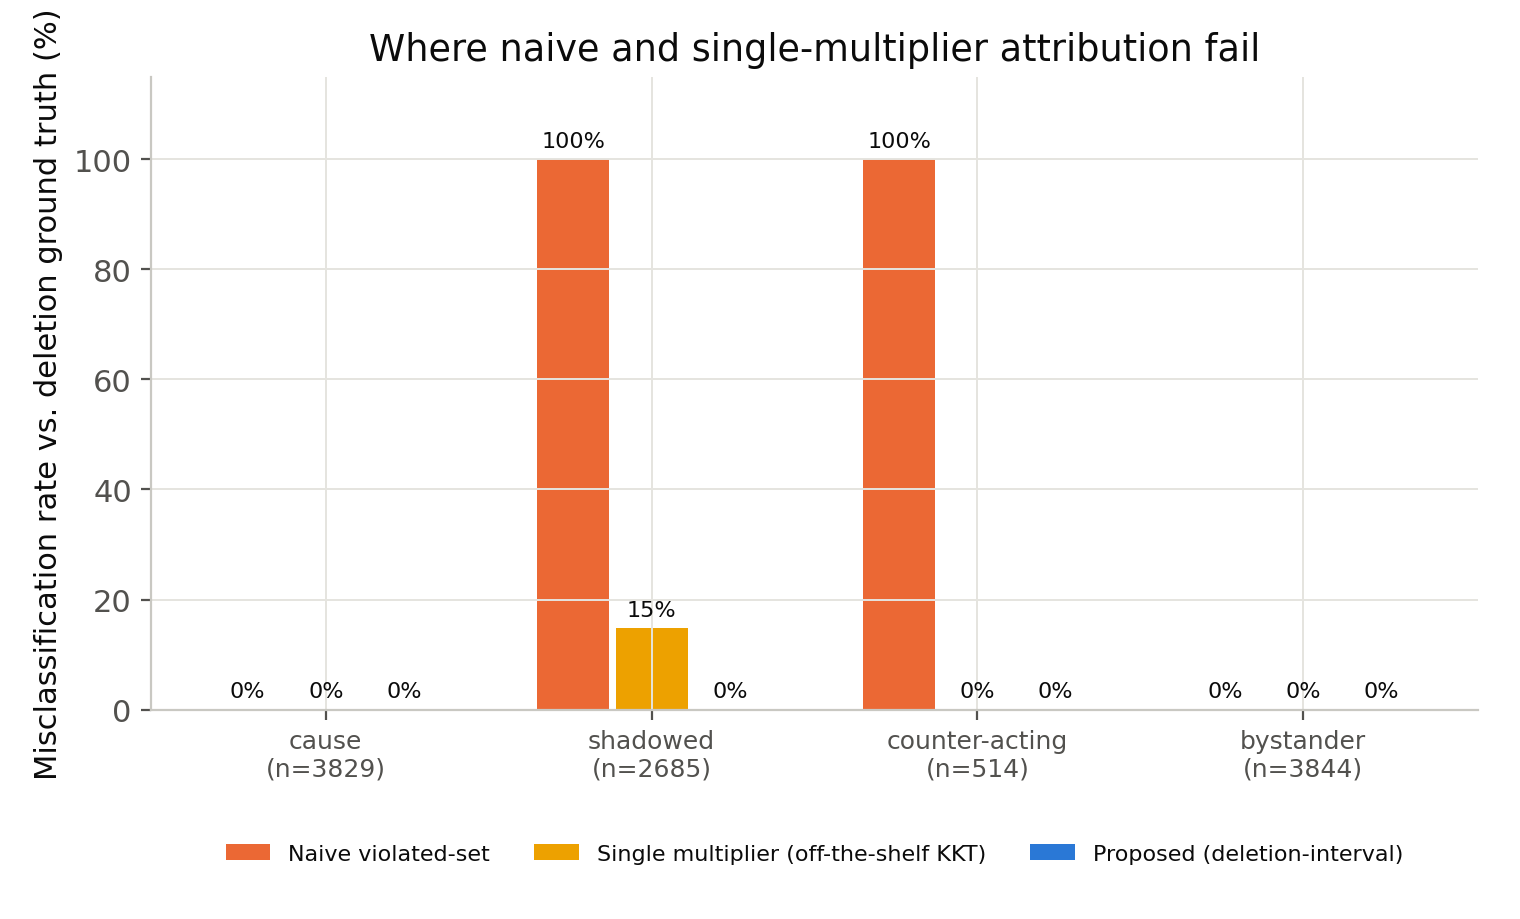
\includegraphics[width=0.85\textwidth]{fig2_taxonomy_errors.png}
\caption{Misclassification rate by taxonomy category. The naive violated-set
rule is wrong on \emph{every single} shadowed instance (2{,}685/2{,}685, it
reports a violated-but-unnecessary constraint as responsible) and on
\emph{every single} counter-acting instance (514/514, it misses a
not-violated-but-necessary constraint entirely). The single-multiplier rule
recovers most of this but still misattributes 15\% of shadowed instances
(the ones with a genuinely non-unique optimal multiplier). The proposed
degeneracy-aware method is exact in all four categories.}
\label{fig:taxonomy}
\end{figure}

\begin{figure}[h]
\centering
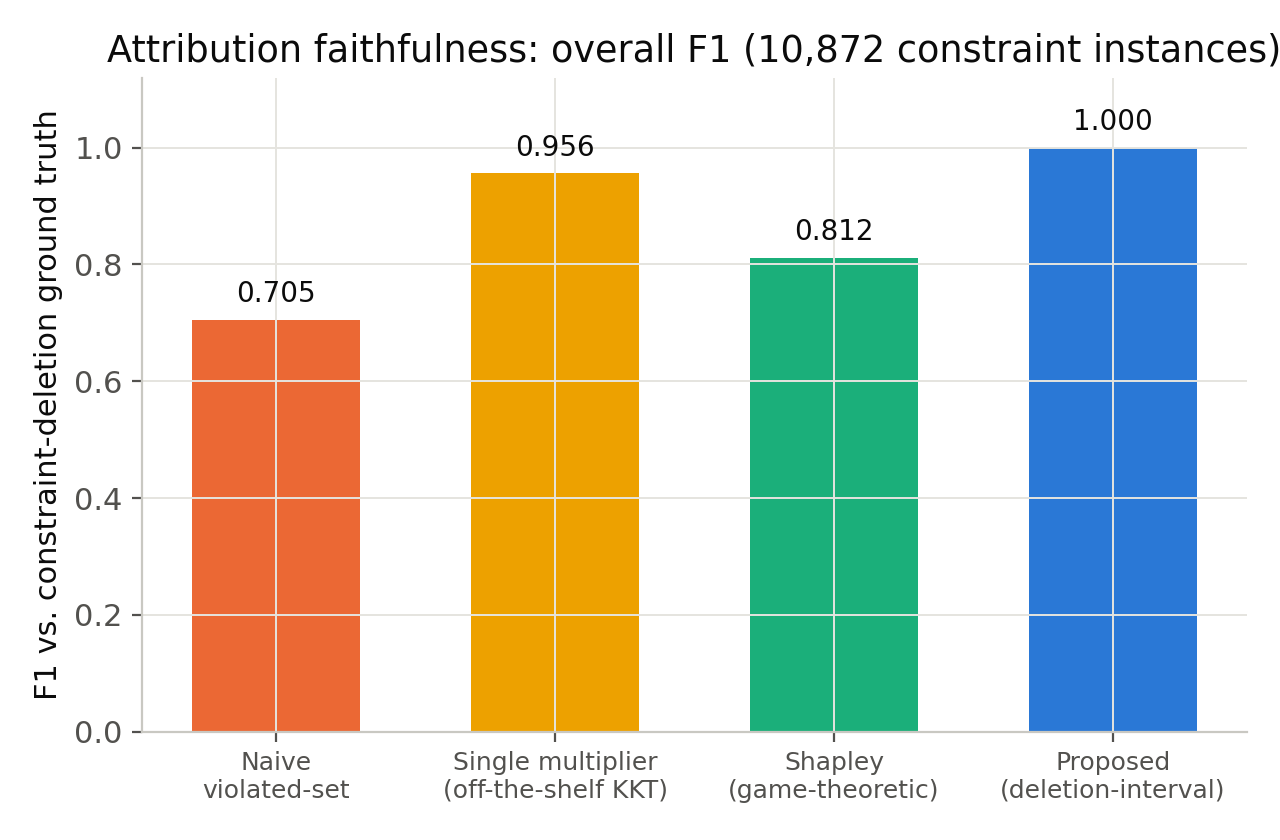
\includegraphics[width=0.75\textwidth]{fig1_attribution_f1.png}
\caption{Overall attribution F1 by method.}
\label{fig:f1}
\end{figure}

\textbf{Interpretation.} This is the sharpest and most publishable result of
the pilot. It is not merely that the proposed method scores $1.000$ (which
follows deductively from Theorem~2, already confirmed in
Sec.~\ref{sec:exp1}); it is \emph{how badly and how systematically the two
realistic incumbent practices fail}, and that the failure mode is exactly
where the paper's taxonomy predicts it: naive violated-set explanations are
maximally wrong on shadowed and counter-acting constraints -- not a rare edge
case but 100\% of $2{,}685{+}514=3{,}199$ such instances in this sample (29\%
of all constraint instances tested). Even a solver's own multiplier output,
taken naively, is wrong 15\% of the time specifically on shadowed constraints,
which is the operationally relevant failure since standard QP solvers do not
report degeneracy. The Shapley baseline, despite using genuine cooperative
game credit rather than a raw multiplier, is \emph{also} wrong on 100\% of
shadowed instances and drags down its overall F1 to 0.812 -- worth noting
explicitly in the paper as it heads off an obvious reviewer question (``why
not just use SHAP''): SHAP-style credit assigns strictly positive value to a
constraint whenever removing it \emph{ever} changes the energy within some
coalition, which is a different (and here, provably wrong) question from
whether removing it changes the \emph{actual optimum}.

% ======================================================================
\section{Experiment 3 --- Certified Counterfactual Explanations}
\label{sec:exp3}

\textbf{Single obstacle, closed form.} The closed-form displacement
$d_{\mathrm{cf}}=R-\|d-c\|$ (Sec.~IV-C of the manuscript) was checked against
an independently derived, purely numerical computation: for 3{,}600 angularly
swept directions, the exact 1-D quadratic root for the minimal positive step
reaching the constraint boundary in that direction was solved directly (no
reuse of the paper's algebra), and the global minimum over directions was
taken as the numerical reference. Across 584 instances where the filter was
active, the closed form matched this independent reference to
$3.5\times10^{-7}$ absolute/relative error, consistent with the angular
sampling resolution ($0.1^\circ$) -- i.e.\ the residual is sampling error in
the \emph{check}, not error in the formula.

\textbf{Multiple obstacles, two-sided certificate.} For 365 multi-obstacle
scenarios (2--4 circular obstacles, shared perturbation of robot position),
the lower bound $d_{\mathrm{lower}}=\max_i d_{\mathrm{cf},i}$ and a certified
feasible upper bound $d_{\mathrm{feasible}}$ (best point found by the same
angular sweep, now enforcing all obstacles simultaneously) were computed.

\begin{table}[h]
\centering
\caption{Two-sided counterfactual certificate, 365 multi-obstacle scenarios.}
\begin{tabular}{lr}
\toprule
Quantity & Value \\
\midrule
Bound $d_{\mathrm{lower}}\le d_{\mathrm{feasible}}$ held & \cellcolor{ok!25}365/365 (100\%) \\
Median relative gap & $8.7\times10^{-8}$ \\
Mean relative gap & 2.0\% \\
90th-percentile relative gap & 2.9\% \\
Maximum relative gap & 61.1\% \\
\bottomrule
\end{tabular}
\end{table}

The bound never failed, which is the minimum bar for calling it a
``certificate.'' The median gap is essentially zero (a single obstacle
dominates in most sampled configurations, so the bound is exact there), but
the tail is not tight: cases with 61\% relative gap occur when two or more
obstacles require displacement in substantially different directions, so no
single-obstacle bound reflects the interaction cost. \textbf{This is a real
limitation to name explicitly in the paper} (Sec.~VI, ``Limitations''
currently does not mention it) rather than leave implicit -- and it is a
natural, scoped algorithmic extension (an SOCP/QCQP-based joint lower bound,
or a Dinkelbach-style improvement, rather than $\max_i$) worth a paragraph in
the paper or a short follow-up.

% ======================================================================
\section{Experiment 4 --- Does the Conditioning Indicator Predict Instability?}
\label{sec:exp4}

\textbf{Setup.} 674 intervening scenarios (a mix of general random and
forced-degenerate instances spanning $\kappa_{\mathrm{stab}}=\sigma_{\min}(M_I)$
from $10^{-19}$ to $0.99$) were each perturbed 25 times with small
($\|\delta b\|=10^{-4}$) random constraint perturbations, with the \emph{full}
QP re-solved (not the linearized system) each time. For perturbations that did
not change the active set, the empirical multiplier sensitivity ratio
$\|\Delta\lambda\|/\|\Delta b\|$ was recorded; the active-set switching rate
was also recorded per scenario.

\begin{figure}[h]
\centering
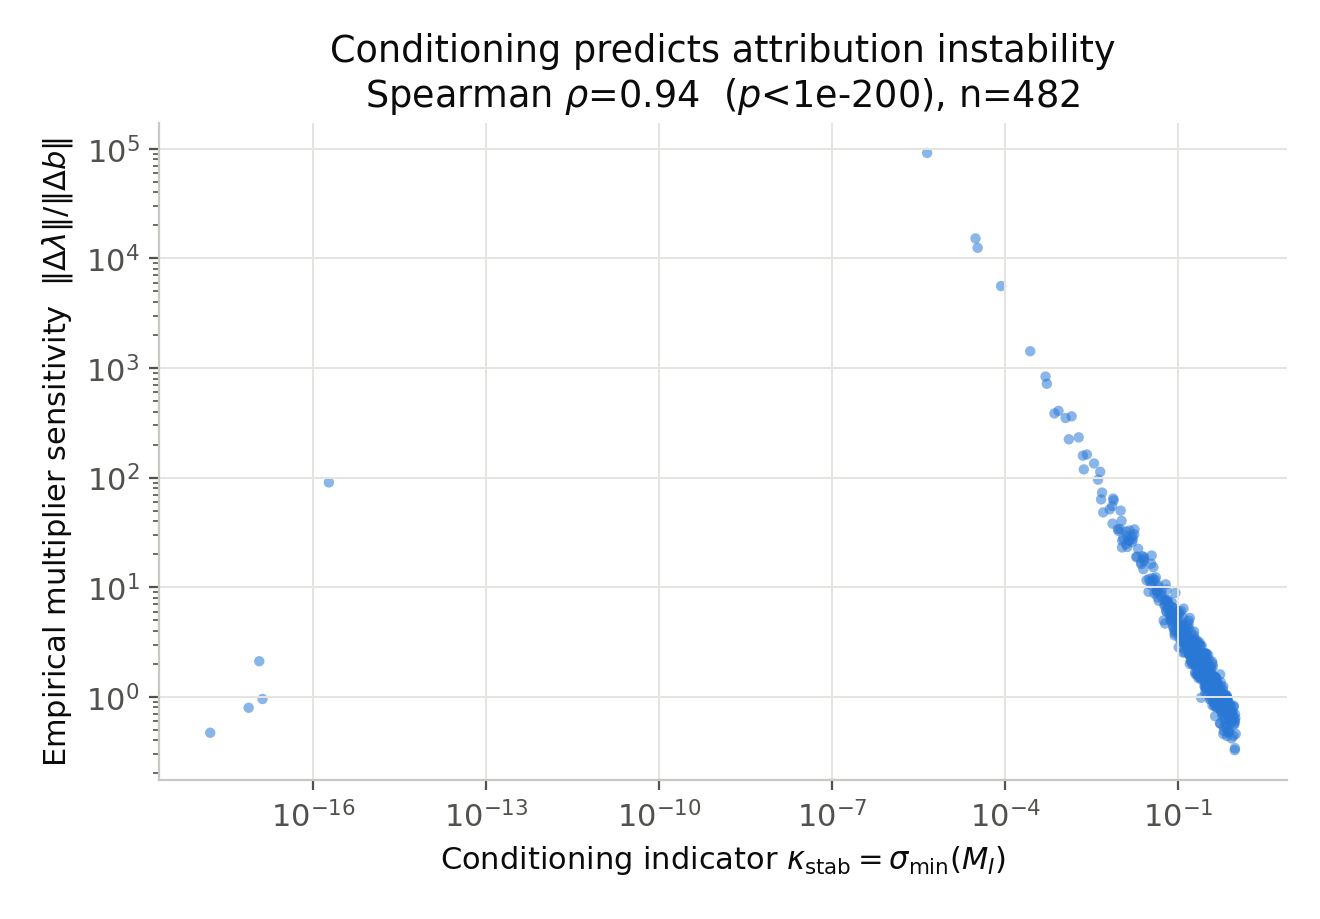
\includegraphics[width=0.72\textwidth]{fig3_stability.png}
\caption{Conditioning indicator vs.\ empirical multiplier sensitivity, 482
scenarios with usable non-switching perturbations. Spearman
$\rho=0.94$ ($p<10^{-200}$).}
\label{fig:stability}
\end{figure}

\begin{table}[h]
\centering
\caption{Conditioning vs.\ instability, Spearman rank correlation.}
\begin{tabular}{lrr}
\toprule
Pair & $\rho$ & $p$ \\
\midrule
$\log(1/\kappa_{\mathrm{stab}})$ vs.\ mean sensitivity ratio & 0.94 & $<10^{-200}$ \\
$\log(1/\kappa_{\mathrm{stab}})$ vs.\ active-set switching rate & 0.79 & $<10^{-140}$ \\
\bottomrule
\end{tabular}
\end{table}

29\% of scenarios experienced at least one active-set switch under a
perturbation of size only $10^{-4}$, confirming that near-degeneracy is not a
rare corner case in these CBF-QP-like instances -- it is common enough
(consistent with the 20.5\% degeneracy rate in Experiment~1) that RQ4 and the
conditioning-indicator reporting mechanism are load-bearing parts of the
system, not a defensive footnote.

% ======================================================================
\section{Cross-Cutting Risks Identified by the Pilot}
\label{sec:risks}

\begin{enumerate}[leftmargin=1.6em]
  \item \textbf{Degeneracy is common, not rare.} $\sim$20--29\% of instances
        in these pilot distributions have a non-unique dual optimum or switch
        active set under a $10^{-4}$ perturbation. The degeneracy-aware
        machinery (attribution intervals, conditioning indicator) is
        therefore central to the method's practical validity, not an edge
        case; it should be emphasized, not hedged, in the paper.
  \item \textbf{Multi-constraint counterfactual certificates can be loose}
        (up to 61\% relative gap in this sample) under constraint
        interaction. This should be an explicit, quantified limitation, and
        is a natural extension for a stronger joint bound.
  \item \textbf{Floating-point precision degrades with conditioning}, exactly
        where the theory predicts. Any production implementation should
        normalize constraint rows (as the manuscript already recommends) and
        should consider a regularized ($M_I+\epsilon I$) multiplier solve
        when $\kappa_{\mathrm{stab}}$ falls below a chosen threshold.
  \item \textbf{The Shapley/SHAP-style comparison is worth keeping in the
        real experiments and in the paper}, because it produces a
        genuinely informative negative result (100\% error on shadowed
        constraints) that pre-empts a predictable reviewer question and is
        cheap to compute for the $p\le 6$ regime realistic for a CBF-QP
        filter.
\end{enumerate}

% ======================================================================
\section{Recommendation}

\textbf{Proceed to the full experiments.} All four pilot questions in
Sec.~1 returned a clear, positive, and in three of four cases statistically
overwhelming answer, with zero falsifying evidence against any of the paper's
theorems or claimed identities across roughly 17{,}000 total test instances.
Equally important for a go/no-go decision: the idea is \emph{cheaply and
decisively testable} -- this entire pilot, covering identity verification,
a four-way attribution comparison including a genuine SHAP-style baseline,
closed-form and certificate counterfactual validation, and a stability/
conditioning study, ran in well under one minute of compute on synthetic
data with no GPU, no simulator, and no robot. That combination (strong
positive signal, low cost of the check) is exactly the profile that justifies
the next, more expensive step: Safety-Gymnasium/MuJoCo experiments with a
learned policy (RQ1--RQ2 at scale, with real policies rather than synthetic
$u_\pi$) and, hardware permitting, the manipulator demonstration.

Two concrete pieces of pre-work are suggested before or alongside the safe-RL
experiments, both directly motivated by this pilot rather than being
generic advice:
\begin{itemize}[leftmargin=1.6em]
\item Add the degeneracy-rate and conditioning-vs-instability results
      (Sec.~\ref{sec:exp1} and \ref{sec:exp4} here) as a short numerical
      subsection in the paper -- they are novel, cheap to reproduce, and
      directly support the paper's degeneracy-handling design decision,
      which a reviewer could otherwise dismiss as over-engineering for a
      rare case.
\item Decide and state explicitly, in the Limitations section, the known
      looseness of the multi-obstacle counterfactual certificate
      (Sec.~\ref{sec:exp3}), with either a quantified bound on the gap or a
      pointer to a joint-bound extension.
\end{itemize}

\vspace{6pt}
\noindent\textit{Reproducibility.} All scenario generators, the exact QP
solver, and the four experiment scripts are included alongside this report
(\texttt{qp\_core.py}, \texttt{scenarios.py}, \texttt{exp1\_identities.py},
\texttt{exp2\_attribution.py}, \texttt{exp3\_counterfactual.py},
\texttt{exp4\_stability.py}, \texttt{make\_plots.py}), together with the raw
result tables (CSV/JSON) underlying every number in this report.

\end{document}
